\chapter{Wymagania funkcjonalne}
\label{Chapter3}

Celem sprawnej realizacji celów warunkujących powstanie systemu \textit{iQuest}, musi on spełniać szereg wymagań funkcjonalnych. Obejmuje to m.in. tworzenie i prowadzenie (zarówno ze strony Ankietera, jak i Respondenta) Badań i Ankiet, a także analizę powstałych na ich podstawie zestawień danych. Ze względu na charakter projektu \textit{iQuest}, niezwykle ważną funkcjonalnością okazał się najbardziej podstawowy ze wszystkich mechanizmów -- logowanie do systemu. Koniecznością jest bowiem prawidłowa autoryzacja użytkowników systemu, jak też współpraca z innymi systemami Uczelni.

\section{Diagram przypadków użycia}
\label{Chapter31}

Na rysunku \ref{rys:UseCaseView} przedstawiono diagram przypadków użycia. W ramach systemu udostępniane są różne funkcje, możliwe do wykonania przez różnych aktorów. Dla przykładu, Ankieter może tworzyć Badania i analizować ich Statystyki oraz Raporty, podczas gdy Respondent może odpowiadać w Ankietach w ramach skierowanych do niego Badań; Administrator zarządza przydzielaniem ról; Administrator Bazy Danych zajmuje zarządza grupami Respondentów i przydzielaniem praw i zezwoleń.

\begin{figure}[H]
\centering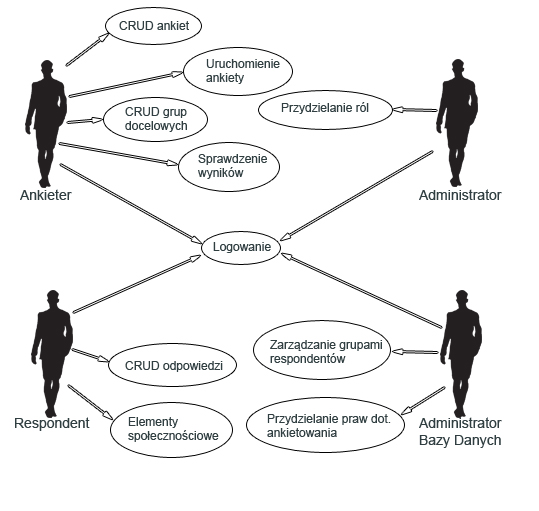
\includegraphics[width=0.9\textwidth]{figures/UseCaseView}
\caption{Diagram przypadków użycia}\label{rys:UseCaseView}
\end{figure}

\section{Ankieter}
\label{Chapter32}

Poniżej przedstawiono przypadki użycia dotyczące Ankietera.

\subsection{UC01: Stworzenie Ankiety}
\label{Chapter321}

\ucsection{UC01: Stworzenie Ankiety}{Ankieter}
{Ankieter jest zalogowany w Systemie i chce utworzyć Ankietę}
{}{\ucactions{
\ucaction{1. Ankieter uruchamia interfejs tworzenia Ankiety. Podaje atrybuty Ankiety: nazwę Ankiety, wstęp, podsumowanie}
\ucaction{2. System prezentuje stronę umożliwiającą dodawanie pytań}
\ucaction{3. Ankieter wybiera typ pytania}
\ucaction{4. Ankieter podaje treść pytania}
\ucaction{5. Ankieter podaje możliwe odpowiedzi}
\ucaction{6. Ankieter akceptuje Ankietę}
\ucaction{7. System prezentuje podsumowanie ankiety i zapisuje ją w Katalogu Ankiet ankietera}
}}
{\ucextensions{
\ucaction{4.A Typ pytania: pytanie otwarte}
\ucaction{4.A.1 Ankieter pomija krok 5.}
\ucaction{6.A Ankieter chce dodać kolejne pytanie}
\ucaction{6.A.1 Powrót do kroku 3.}
}}
{}

\subsection{UC02: Edycja Ankiety}
\label{Chapter322}

\ucsection{UC02: Edycja Ankiety}{Ankieter}
{
1. Ankieta znajduje się w Systemie i jest dostępna dla Ankietera \\
2. Ankieta nie jest częścią czynnego Badania \\
3. Ankieter jest zalogowany w Systemie i chce zmodyfikować istniejącą Ankietę
}
{}{\ucactions{
\ucaction{1. Ankieter wybiera Ankietę do modyfikacji}
\ucaction{2. System prezentuje wskazaną Ankietę}
\ucaction{3. Ankieter modyfikuje lub usuwa dostępne pytania}
\ucaction{4. Ankieter potwierdza chęć zapisu zmienionej Ankiety}
\ucaction{5. System zapisuje zmienioną Ankietę}
}}
{\ucextensions{
\ucaction{3.A. Edycja możliwych odpowiedzi do pytań}
\ucaction{3.A.1 Ankieter edytuje możliwe odpowiedzi do pytań}
}}
{}

\subsection{UC03: Wybór Grupy Docelowej}
\label{Chapter323}

\ucsection{UC03: Wybór Grupy Docelowej}{Ankieter, Administrator}
{
1. Ankieta znajduje się w Systemie i jest dostępna dla Ankietera \\
2. Grupa Docelowa znajduje się w Systemie i jest dostępna dla Ankietera \\
3. Ankieter jest zalogowany w Systemie i chce wybrać Grupę Docelową
}
{}{\ucactions{
\ucaction{1. Ankieter wybiera opcję tworzenia Badania}
\ucaction{2. System prezentuje listę Grup Docelowych, do których Ankieter ma uprawnienia}
\ucaction{3. Ankieter wybiera Grupy Docelowe dla danego Badania}
\ucaction{4. Ankieter akceptuje powiązanie Grup Docelowych z Ankietą}
}}
{\ucextensions{
\ucaction{3.A. Zawężenie Grupy Docelowej}
\ucaction{3.A.1 Ankieter wybiera członków Grupy Docelowej, do której ma być skierowana Ankieta.}
\ucaction{3.A.2 Powrót do kroku 4.}
\ucaction{3.B. Grupa Docelowa poszukiwana przez Ankietera nie istnieje}
\ucaction{3.B.1 Ankieter próbuje połączyć kilka Grup Docelowych lub ich fragmentów}
\ucaction{3.B.2 W przypadku niepowodzenia kroku rozszerzenia 3.B.1, bądź wystąpienia takiej konieczności, Ankieter informuje Administratora, że nie ma praw do wysyłania ankiet do wskazanych osób i/lub powiadamia go (za pomocą poczty elektronicznej) o potrzebie stworzenia Grupy Docelowej o konkretnych atrybutach (BC03)}
\ucaction{3.B.3 W przypadku pominięcia kroku rozszerzenia 3.B.2, powrót do kroku 4., w przeciwnym razie, powrót do kroku 1.}
}}
{}

\subsection{UC04: Uruchomienie Badania}
\label{Chapter324}

\ucsection{UC04: Uruchomienie Badania}{Ankieter, Respondent}
{
1. Ankieta znajduje się w Systemie i jest dostępna dla Ankietera \\
2. Ankieta jest powiązana z Grupą Docelową \\
3. Ankieter jest zalogowany w Systemie i chce rozesłać istniejącą Ankietę
}
{Respondenci powiadomieni o Ankiecie}{\ucactions{
\ucaction{1. Ankieter ustawia czas rozpoczęcia i zakończenia Badania oraz grupę docelową (UC3)}
\ucaction{2. Ankieter potwierdza chęć uruchomienia Badania}
\ucaction{3. System udostępnia Ankietę Respondentom}
\ucaction{4. System powiadamia Respondentów o Ankiecie}
}}
{\ucextensions{
\ucaction{1.A. Ankieter chce prowadzić cykliczną ankietyzację}
\ucaction{1.A.1 Ankieter ustawia częstotliwość powtarzania Badania}
}}
{}

\subsection{UC06: Sprawdzenie wyników}
\label{Chapter325}

\ucsection{UC06: Sprawdzenie wyników}{Ankieter}
{
1. Ankieta znajduje się w Systemie, zawiera odpowiedzi od Grupy Docelowej i jest dostępna dla Ankietera \\
2. Ankieter jest zalogowany w Systemie i chce pozyskać informacje od Studentów/Absolwentów
}
{Wygenerowany Raport}{\ucactions{
\ucaction{1. Ankieter wybiera Ankietę, której wyniki chce poznać}
\ucaction{2. Ankieter wybiera typ Raportu, który chciałby zobaczyć}
\ucaction{3. System generuje i wyświetla Raport}
}}
{}

\section{Respondent}
\label{Chapter33}

Poniżej przedstawiono przypadki użycia dotyczące Respondenta.

\subsection{UC05: Udzielenie odpowiedzi}
\label{Chapter331}

\ucsection{UC05: Udzielenie odpowiedzi}{Respondent}
{
1. Respondent dostaje powiadomienie o Ankiecie (link bezpośredni do Ankiety) \\
2. Respondent jest zalogowany w Systemie i chce wypełnić Ankietę
}
{}{\ucactions{
\ucaction{1. Respondent wybiera Ankietę, w której chce wziąć udział}
\ucaction{2. System prezentuje wybraną Ankietę Respondentowi}
\ucaction{3. Respondent udziela odpowiedzi na pytania}
\ucaction{4. Respondent zatwierdza wypełnioną Ankietę}
\ucaction{5. System zapisuje odpowiedzi}
}}
{\ucextensions{
\ucaction{2.A. Przedawniona Ankieta}
\ucaction{2.A.1 System informuje, że Ankieta już się zakończyła}
\ucaction{5.A. Brak odpowiedzi na niektóre pytania}
\ucaction{5.A.1 System pozwala powrócić do pytań, na które nie udzielono odpowiedzi}
\ucaction{5.A.2 Powrót do kroku 1.}
}}
{}

\section{Administrator}
\label{Chapter34}

Poniżej przedstawiono przypadki użycia dotyczące Administratora.

\subsection{UC07: Tworzenie Grupy Docelowej}
\label{Chapter341}

\ucsection{UC07: Tworzenie Grupy Docelowej}{Administrator}
{
1. Ankieter chce wysyłać Ankiety do określonych Respondentów w prosty sposób \\
2. Administrator jest zalogowany w Systemie i chce utworzyć nową Grupę Docelową
}
{Nowa Grupa Docelowa w Systemie}{\ucactions{
\ucaction{1. Administrator wybiera opcję tworzenia Grup Docelowych}
\ucaction{2. System prezentuje formularz tworzenia Grupy Docelowej}
\ucaction{3. Administrator wprowadza nazwę tworzonej Grupy Docelowej, wybiera Grupę Nadrzędną oraz Respondentów do dodania do Grupy Docelowej}
\ucaction{4. Administrator potwierdza chęć stworzenia Grupy Docelowej}
\ucaction{5. System zapisuje nową Grupę Docelową}
}}
{\ucextensions{
\ucaction{4.A Brak Grupy Nadrzędnej}
\ucaction{4.A.1 Administrator Bazy Danych nie uzupełnia Grupy Nadrzędnej}
}}
{}

\subsection{UC08: Edycja Grupy Docelowej}
\label{Chapter342}

\ucsection{UC08: Edycja Grupy Docelowej}{Administrator}
{
1. Grupa Docelowa znajduje się w Systemie \\
2. Administrator jest zalogowany w Systemie i chce zmodyfikować Grupę Docelową
}
{Zmodyfikowana lista członków Grupy Docelowej}{\ucactions{
\ucaction{1. Administrator wybiera Grupę Docelową}
\ucaction{2. Administrator wybiera członka\slash członków Grupy Docelowej do edycji\slash usunięcia}
\ucaction{3. Administrator dodaje\slash edytuje]\slash usuwa członka\slash członków Grupy Docelowej}
\ucaction{4. Administrator potwierdza chęć wprowadzenia zmian}
\ucaction{5. System zapisuje zmiany}
}}
{}

\section{Wszyscy Użytkownicy}
\label{Chapter35}

Poniżej przedstawiono przypadki użycia dotyczące wszystkich Użytkowników.

\subsection{UC09: Logowanie do Systemu}
\label{Chapter351}

\ucsection{UC09: Logowanie do Systemu}{Użytkownik (Ankieter, Administrator, Respondent)}
{Użytkownik posiada konto w Systemie i posiada poprawne dane logowania}
{Użytkownik jest zalogowany w Systemie}{\ucactions{
\ucaction{1. System wyświetla Użytkownikowi formularz logowania}
\ucaction{2. Użytkownik podaje login lub adres e-mail oraz hasło}
\ucaction{3. System uwierzytelnia Użytkownika}
}}
{\ucextensions{
\ucaction{2.A Użytkownik chce się zalogować przy pomocy eKonta}
\ucaction{2.A.1 Użytkownik wybiera opcję logowania przez eKonto}
\ucaction{2.A.2 System przekierowuje Użytkownika na stronę logowania przez eKonto (eLogin)}
\ucaction{2.A.3 Użytkownik wprowadza dane logowania do eKonta}
\ucaction{2.A.4 Powrót do kroku 3.}
}}
{}